\documentclass[a4paper,11pt]{article}

\usepackage{packageINSA}

\usepackage{float}
\usepackage{wrapfig}
\usepackage{graphicx} %%For loading graphic files
\usepackage{subfig} %%Subfigures inside a figure
\usepackage{pdfpages}
\usepackage{eurosym}
\usepackage{listings}
\usepackage[numbered,framed]{matlab-prettifier}
\usepackage{url}
\usepackage{glossaries}[toc]
\usepackage{lmodern} %Type1-font for non-english texts and characters
\usepackage{lipsum}

\usepackage{amsmath}
\usepackage{amsthm}
\usepackage{amsfonts}
\usepackage{siunitx}
\usepackage[a4paper, total={6in, 8in}]{geometry}


\widowpenalty=10000
\clubpenalty=10000

\setlength{\tabcolsep}{0.5em} % for the horizontal padding
{\renewcommand{\arraystretch}{1.3}% for the vertical padding

\begin{document}
\pagestyle{plain}

% LES DIFFERENTS CHAMPS DE LA COUVERTURE
\sautverticalnegatif{1.4}
% Valeur en cm du saut vertical négatif (ie. vers le haut)
% Modifier cette valeur si le prénom et le nom de l'auteur ne sont pas positionnés au bon endroit par rapport à la ligne "Projet de Fin d'Etudes"
% Si le prénom et le nom tiennent sur la ligne, laisser valeur = 1.4
\specialite{EII}  % Nom de la spécialité
\anneeuniversitaire{2018 - 2019}  % Année universitaire
\titre{Emulateur de la console NES}  % sujet du PFE
\correspondantINSA{Alexandre}{TISSIER}  % Prénom et nom du correspondant INSA
\datesout{27/05/2019}  % Date de la soutenance du PFE

\makeTitlePage % Page de titre / première page

\clearpage

\fontfamily{lmodern}
\selectfont

\tableofcontents

\clearpage

\section{Présentation du projet}
\subsection{Introduction}

Ce projet porte sur l'émulation en langage C du système de la console de jeux vidéo NES (Nintendo Entertainment System), sortie en France en 1987 et développée par la société japonaise Nintendo. Plus spécifiquement, ce projet cherche à \emph{reproduire le comportement} de la console de manière \emph{logicielle} dans le but de jouer sur un ordinateur personnel aux jeux existants. Pour cela, on se fixe plusieurs objectifs :
\begin{itemize}
  \item Émuler le fonctionnement de la NES et se rapprocher au plus près du fonctionnement hardware (émulation précise, voir section \ref{subsec:precision_sur_lemulation})
  \item Connecter le clavier à l'émulateur en tant que périphérique d'entrée et rendre les touches configurables (support de deux joypads)
  \item Pouvoir jouer aux jeux développés sur des cartouches avec un mapper NROM
  \item Être en capacité de redimensionner la fenêtre de jeux.
  \item Avoir des performances fluides (NTSC - 60 FPS)
  \item Développer pour fonctionner sous Linux
\end{itemize}

\subsection{Fonctionnement interne de la NES}
\label{subsec:fonctionnement_interne_nes}

On distingue trois composants principaux constituant la NES :
\begin{itemize}
\item la \emph{CPU} qui est un processeur 6502 8-bit, muni de 56 instructions et de 12 modes d'adressages ainsi que d'un Program Counter (PC) de 16 bits et 5 registres 8-bit (Stack Register, Processor Status, Accumulator, X Register, Y Register). Il adresse donc un domaine de 64 kB détaillé ci-dessous :

\begin{center}
\begin{tabular}{|c|c|c|}
  \hline
  Plage d'adresse & Taille & Utilisation \\
  \hline
  \$0000-\$07FF & \$0800 & 2KB RAM interne\\
  \hline
  \$0800-\$1FFF & \$1800 & Miroirs de \$0000-\$07FF \\
  \hline
  \$2000-\$2007 & \$0008 & Registres de la PPU \\
  \hline
  \$2008-\$3FFF & \$1FF8 & Miroirs de \$2000-2007 \\
  \hline
  \$4000-\$4017 & \$0018 & Registres I/O et APU \\
  \hline
  \$4018-\$401F & \$0008 & Inutilisés \\
  \hline
  \$4020-\$FFFF & \$BFE0 & Espace réservé à la cartouche de jeux \\
  \hline
\end{tabular}
\end{center}
\hspace{1pt}
\item la \emph{PPU} (Picture Processing Unit), la carte vidéo qui génère un signal vidéo composite de 240 lignes de 256 pixels. Son fonctionnement est parallèle et indépendant de la CPU et elle possède son propre espace d'adressage de 8 kB de ROM et 2 kB de RAM pour l'affichage graphique. Elle est également reliée à la CPU par 8 registres dans la plage \$2000-\$2007.
\item l'\emph{APU} (Audio Processing Unit), la carte audio de la NES, qui ne sera pas émulée du fait de la longueur de son implémentation.
\end{itemize}

L'APU ainsi que les périphériques externes sont reliés dans la mémoire de la CPU dans la plage \$4000-\$4017.

\subsection{Précisions sur l'émulation}
\label{subsec:precision_sur_lemulation}
Au vu des performances des processeurs actuels, nous choisissons d'émuler la NES de façon \emph{précise (accurate)}, c'est-à-dire exécuter les composants à chaque instant de l'émulation, ce qui rapproche du fonctionnement machine.
Nous utiliserons la bibliothèque SDL1.2 afin de créer un environnement graphique où afficher le résultat de notre émulation.


\section{Organisation du travail}
\paragraph{}

Simuler logiciellement le comportement d'un appareil tel que la NES nécessite de connaître précisément le fonctionnement de chacune des unités de traitement qui le constitue : leur architecture matérielle, les données qu'elles manipulent, les connexions entre ces différentes unités, etc. La NES jouissant d'une grande popularité, de nombreux développeurs et hackers se sont intéressés à son fonctionnement tant et si bien qu'une communauté de passionnés à vu le jour : \emph{NESDev}. Celle-ci propose, sur son Wiki, des informations détaillées sur l'architecture et le comportement de la machine.

Nous avons donc commencé ce projet par une phase collective de recherche sur le fonctionnement global de la NES afin d'acquérir une vision d'ensemble du système à émuler. Cela nous a permis d'acquérir un socle commun de connaissances sur le sujet.

C'est suite à ces recherches que nous avons pu établir une architecture logicielle appropriée puis une répartition des tâches au sein du groupe. Afin que chaque membre du projet se sente impliqué, cette répartition fut réalisée suivant les préférences de chacun. L'organisation des ressources humaines et temporelles furent retranscrites en un diagramme de Gantt. Sur ce diagramme ainsi que dans le cahier des charges, deux versions du projet ont été prévues : la première (v0) comportant les fonctions vitales à l'émulateur et une seconde (v1) ajoutant des fonctionnalités additionnelles.

Sur toute sa durée, ce projet fut ponctué de réunions d'équipe mais également de séances de travail de groupe, plus conséquentes, effectuées en amont de chaque grande étape du projet. Ces sessions de travail consistaient en une recherche d'informations approfondies sur les futures tâches pour que chacun ait une pleine compréhension des fonctionnalités a développer.

\begin{figure}[h]
   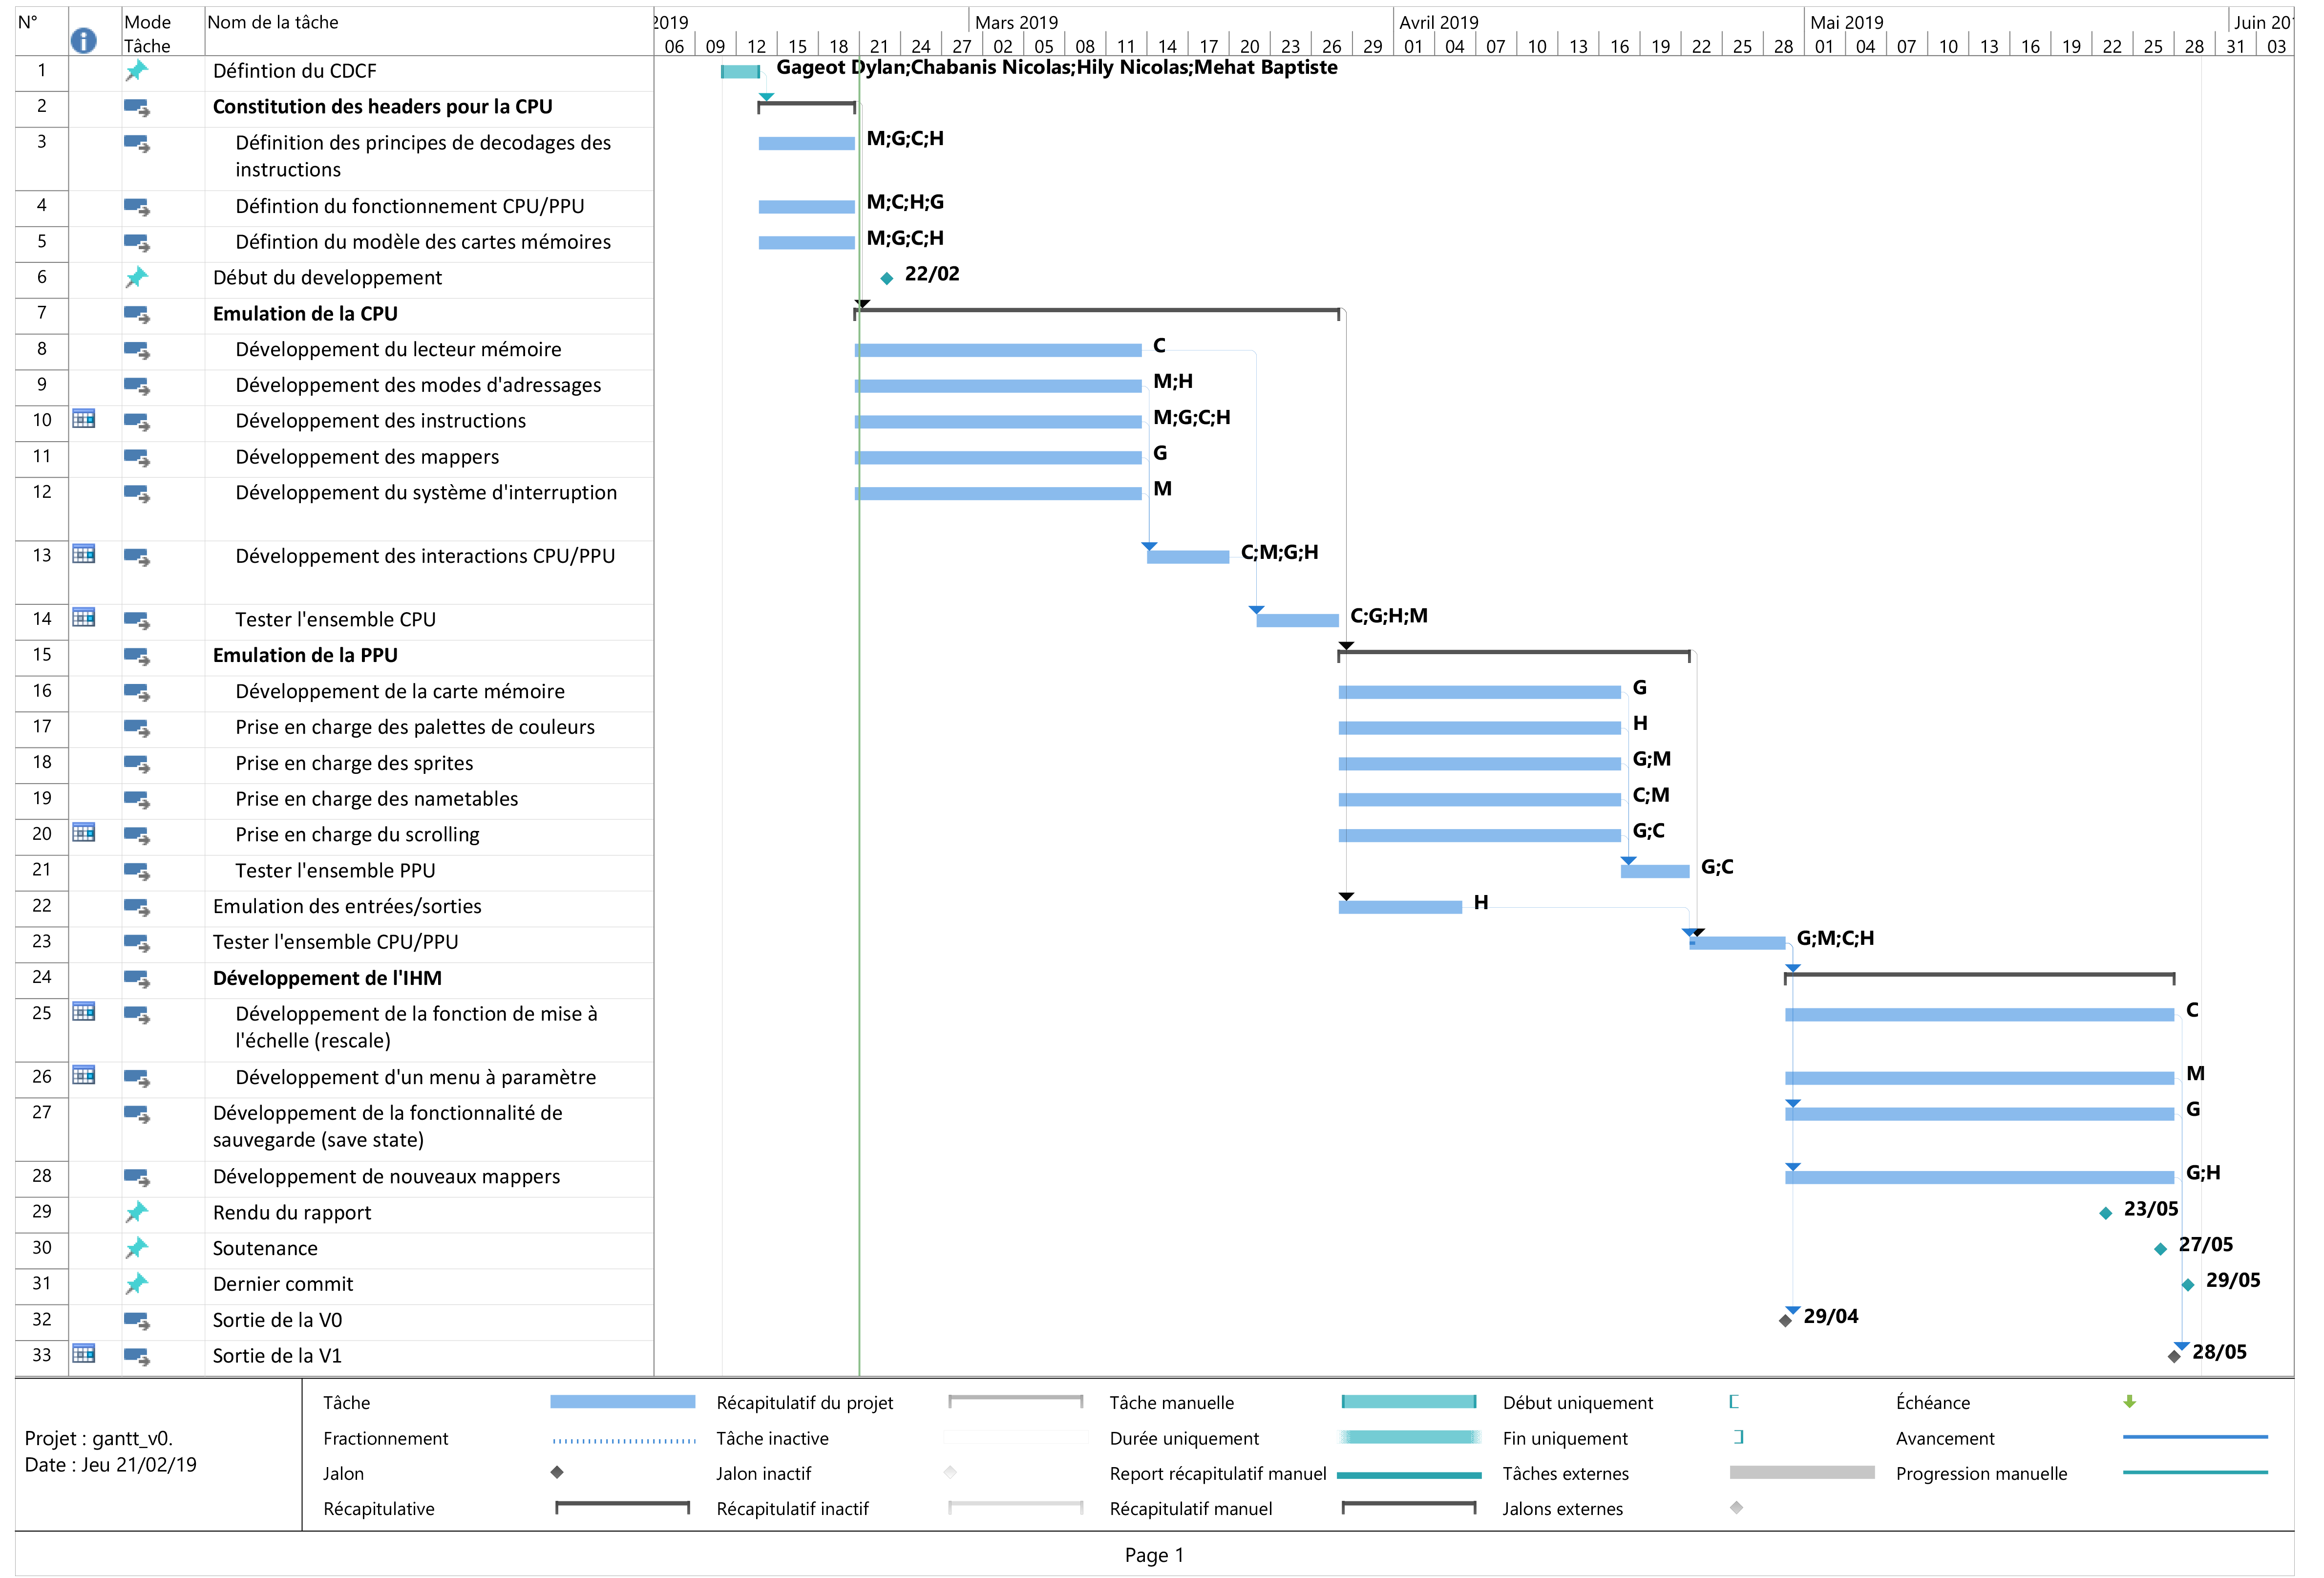
\includegraphics[scale=0.45]{GanttV1.png}
   \caption{\label{étiquette} Diagramme de Gantt de début de Projet}
\end{figure}


\section{Architecture logicielle et moyens de test}
\subsection{Description du concept}

\paragraph{}
La problématique principale du projet fut de concevoir une architecture logicielle qui reflète le fonctionnement de la console mais qui puisse aussi être modulaire. En effet, les composants de la NES communiquent les un avec les autres à travers l'espace d'adressage du processeur 6502, la cartouche de jeu y compris. Avec le format cartouche, il est tout à fait possible de moduler le circuit électronique de la cartouche pour augmenter la capacité de stockage du programme ou sauvegarder des parties. Nous constatons alors que l'espace d'adressage varie d'un type de cartouche (ou \emph{mapper} dans le langage technique de la console) à un autre.

\paragraph{}
Nous avons donc développé notre émulateur sur un modèle orienté objet : chaque structure est accompagnée de fonctions constructrice, destructrice et fonctionnelles. Ce modèle nous permet de gagner en modularité : lors d'un chargement de ROM, venir charger l'espace mémoire correspondant au mapper du jeu et ce de manière transparente pour le reste du système. Vous retrouvez sur la figure \ref{fig:struct_app} l'architecture de l'émulateur du point de vue des structures. La structure \emph{NES} contient le modèle de l'émulateur, incluant la structure \emph{CPU}, \emph{PPU} et \emph{Controller}. Toutes ces structures partagent un même pointeur sur la structure \emph{Mapper}, une structure que l'on pourrait décrire comme une classe abstraite en POO puisqu'elle permet au reste du logiciel de s'abstraire du type de mapper utilisé. Comme toutes classes abstraites, il faut définir le comportement de chaque mapper sur la base des fonctions définies. Dans le délai imparti par le projet, nous n'avons pu décrire que le mapper \emph{NROM}, mais il est tout à fait possible d'agrémenter l'émulateur en mapper avec cette architecture logicielle.

\begin{figure}[H]
	\centering
  \subfloat[Structure \emph{App}]{
    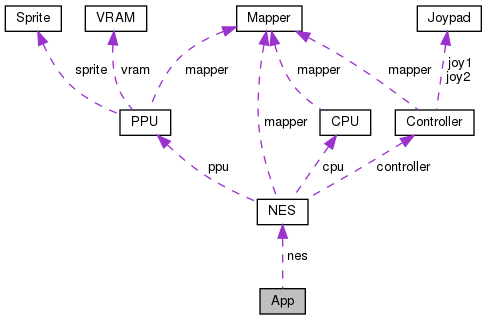
\includegraphics[width=0.45\linewidth]{images/struct_app}
    \label{fig:struct_app}
  }
  \hspace{2cm}
  \subfloat[Structure \emph{MapNROM}]{
    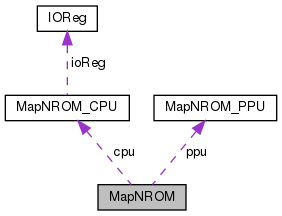
\includegraphics[width=0.25\linewidth]{images/struct_map_nrom}
    \label{fig:struct_map_nrom}
  }
  \caption{Structures de l'émulateur}
  \label{fig:structure}
\end{figure}

\paragraph{}
La fonction NES\_NextFrame() est la fonction de plus haut niveau qui permet d'émuler l'ensemble de la NES jusqu’à ce qu'une image soit produite. Nous sommes en capacité de forcer l'émulation à la vitesse adéquate en forçant 60 images par secondes dans l'applicatif. L'application est assurée par le module App, permettant de lier le modèle (module NES) avec la vue et le contrôleur (assurés par la SDL).

\subsection{Moyens de tests}

En plus des tests unitaires, nous avions à disposition des ROMs permettant de tester la conformité de notre émulation. Ces ROMs se trouvent sur \url{nesdev.com}, tout comme les informations sur le fonctionnement de la console sur lequel nous nous sommes basés. Pour tester le bon fonctionnement du processeur 6502, nous exécutons puis comparons les logs que nous avons produits avec celui fourni par un programme spécifique. Pour le test de la PPU, les jeux \emph{Donkey Kong} et \emph{Super Mario Bros} nous ont permis de tester les différentes spécificités et cas à difficultés.


\section{Conclusion}
Ce projet de C a été très enrichissant d'un point de vue travail de groupe, organisationnel et intellectuel. Étant le premier projet a réaliser à quatre sur notre temps personnel, cela n'a pas été facile d'aménager nos emplois du temps. Ce projet s'est finalement très bien déroulé. Lors de nombreuses réunions, le travail a été défini, expliqué et réparti, selon nos forces et nos faiblesses. De plus, nous avons pu mettre en application et développer toutes les connaissances vues en Langage C, Méthodologie Conception Logicielle et même Architectures des calculateurs. Pour finir, ce projet nous laisse encore de grandes possibilités d'évolutions comme par exemple le codage de l'APU, de l'IHM, le développement de nouveaux mappers et la mise en place de fonctions telle que la sauvegarde. Nous estimons un total d'environ cinq à six mois pour coder l'intégralité de ces fonctions. Il faudrait un mois pour l'APU ainsi qu'un autre pour l'IHM. Le développement des mappers serait plus long. En effet, il s'agirait de rendre notre émulateur capable de lire quatre à cinq autres types de cartouches NES. Cela permettrait de pouvoir jouer à une grande majorité dess jeux. De plus, l'émulateur demande beaucoup de ressources au processeur. Il est difficile de tenir les 60 FPS sur certaines machines. Il serait donc nécessaire de l'optimiser avec une technique de prédiction, c'est à dire émuler un composant à un moment $t$ que si celui-ci a été ciblé par le programme en exécution sur le 6502.

\begin{figure}[H]
  \centering
   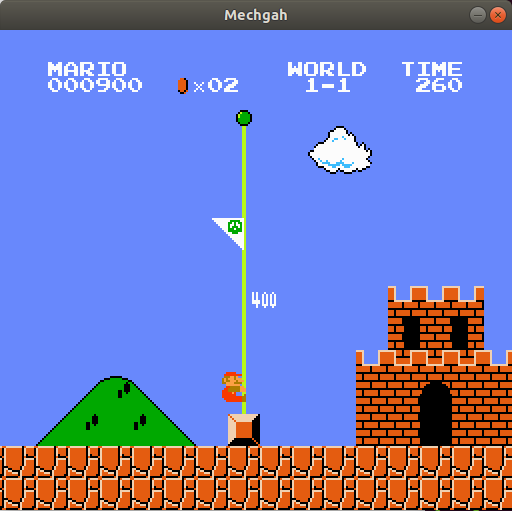
\includegraphics[width=0.50\linewidth]{images/smb_nes.png}
   \caption{Capture d'écran de l'émulateur sur le jeu \emph{Super Mario Bros}}
   \label{fig:gantt_fin}
\end{figure}


\makeAbstractPage
\pagestyle{empty}
\end{document}
